\documentclass[a4paper,11pt]{article}

\usepackage[french]{babel}
\usepackage[T1]{fontenc}
\usepackage[utf8]{inputenc}
\usepackage{graphicx}
%\usepackage{fullpage}

\begin{document}

\title{\textbf{Compte rendu du TP \no 3}\\Spécification d'histogramme}
\author{Thibaut Castanié\\\textit{Master IMAGINA}}
\date{\today}

\maketitle
\thispagestyle{empty}

\newpage 

\section{Expansion dynamique}
\paragraph{Black.pgm} En effectuant une expansion dynamique sur l'image qui semble noire au premier abord, on obtient une image avec une scène visible.
\\J'ai obtenu les valeurs $\alpha$ = 0 et $\beta$ = 13

\begin{center}
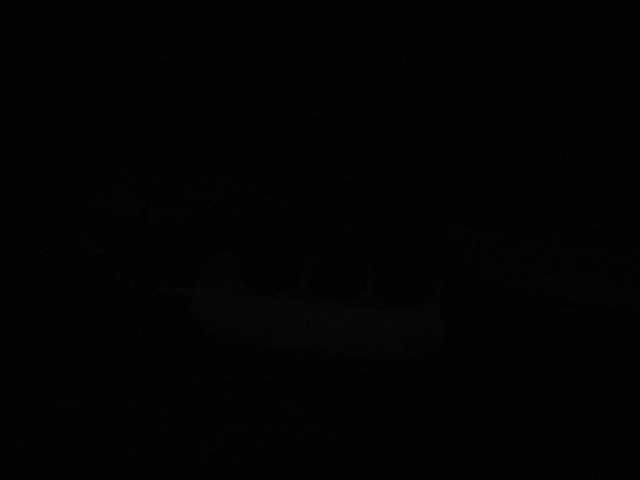
\includegraphics[scale=0.5]{blackgris.png}
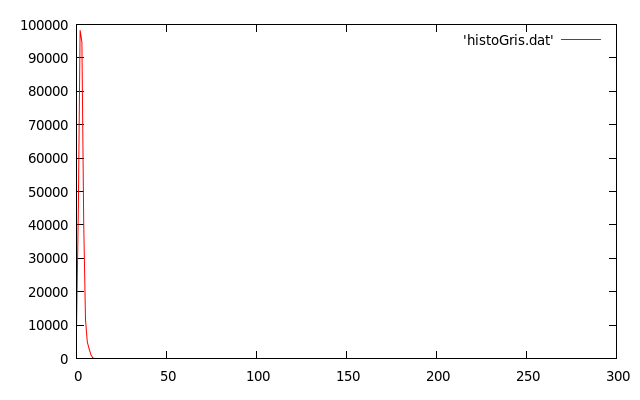
\includegraphics[scale=0.5]{histoBlackGris.png}\\
\textit{L'image black.pgm et son histogramme}\\
\includegraphics[scale=0.5]{blackExpandgris.png}
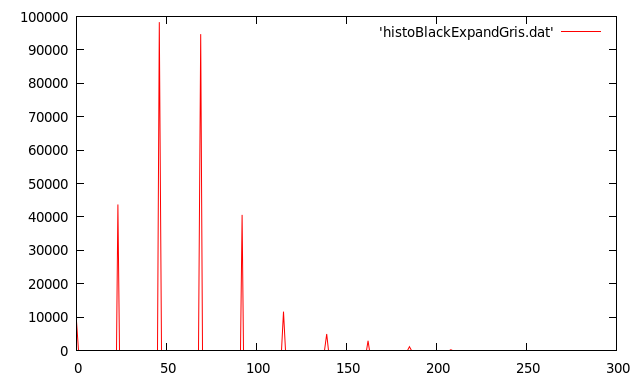
\includegraphics[scale=0.5]{histoBackExpandGris.png}\\
\textit{L'image black.pgm après expansion dynamique, et son histogramme}
\end{center}

\paragraph{Black.ppm} La même opération a été effectuée sur l'image en couleur.\\
$\alpha$R = $\alpha$G = $\alpha$B = 0.\\
$\beta$R = 14, $\beta$G = 13, $\beta$B = 13.

\begin{center}
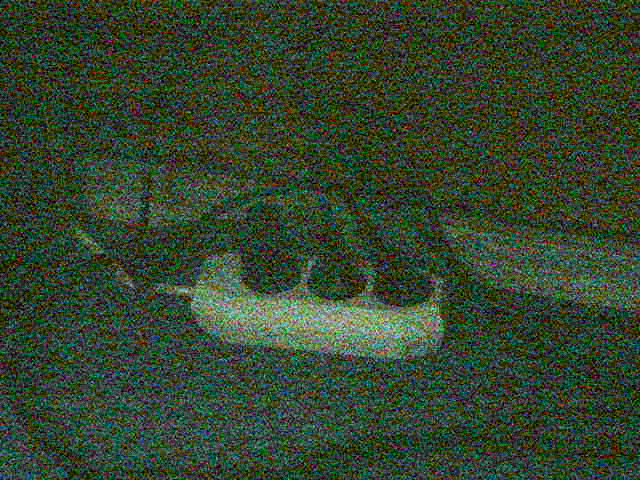
\includegraphics[scale=0.5]{blackexpandcouleur.png}
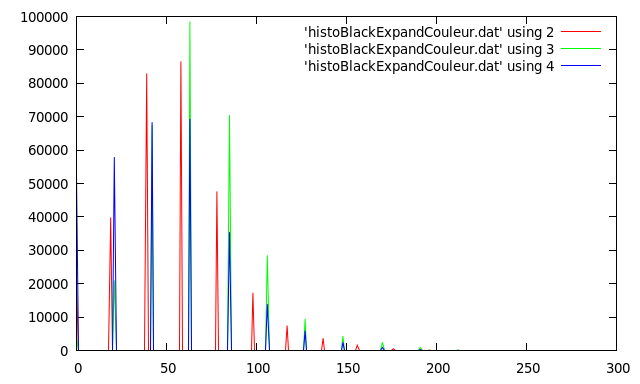
\includegraphics[scale=0.5]{histoBackExpandCouleur.png}\\
\textit{L'image black.ppm après expansion dynamique, et son histogramme}
\end{center}

\newpage
\section{Seuillage des extrema des trois histogrammes}
\paragraph{} L'ensemble des opérations de cet exercice ont étés effectuées sur l'image gimli.ppm ci-dessous. Sur les histogrammes, les couleurs représentent les couleurs réelles de l'image (rouge, vert et bleu).

\begin{center}

\includegraphics[scale=0.5]{gimli.png}
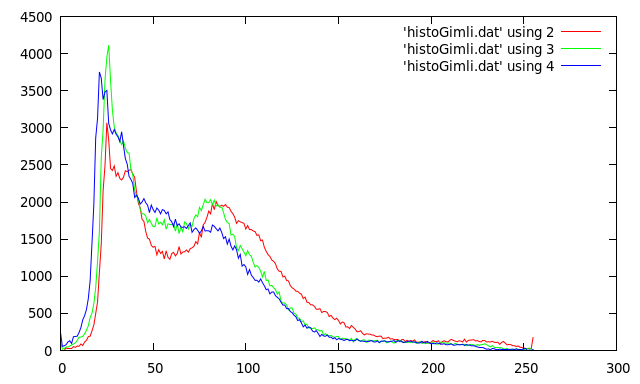
\includegraphics[scale=0.5]{histoGimli.png}\\
\textit{L'image gimli.ppm originale, et son histogramme}
\end{center}

\newpage
\paragraph{Seuillage} Le seuillage consiste à mettre tous les pixels, d'une image couleur, ayant une valeur extrême à une valeur moins extrême ("moins blanc" ou "moins noir").

\begin{center}

\includegraphics[scale=0.5]{gimliseuil.png}
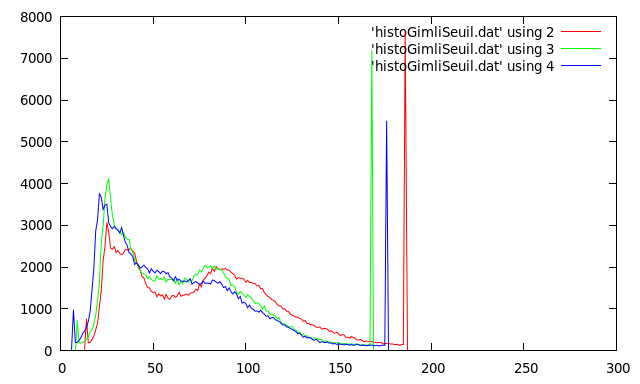
\includegraphics[scale=0.5]{histoGimliSeuil.png}\\
\textit{L'image gimli.ppm seuillée, et son histogramme}
\end{center}

\newpage
\paragraph{Expansion dynamique} On peut ensuite appliquer une expansion dynamique sur l'image ainsi seuillée.

\begin{center}

\includegraphics[scale=0.5]{gimliseuilexpand.png}
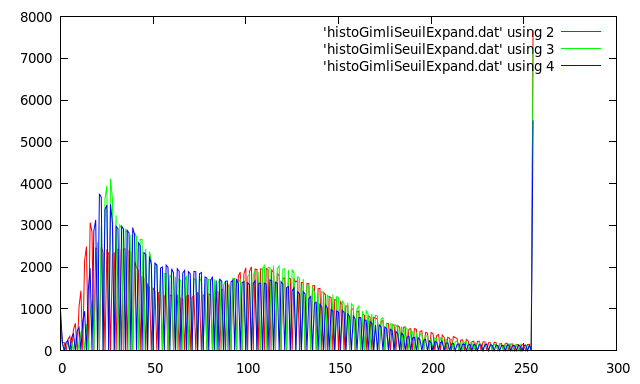
\includegraphics[scale=0.5]{histoGimliSeuilExpand.png}\\
\textit{L'image gimli.ppm après seuillage et expansion, et son histogramme}
\end{center}

\newpage
\section{Égalisation d'histogramme}
\begin{center}

\includegraphics[scale=0.5]{gimli_pgm.png}
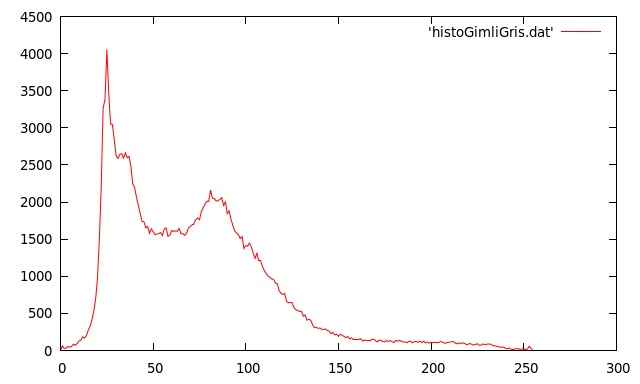
\includegraphics[scale=0.5]{histoGimliGris.png}\\
\textit{L'image gimli.pgm originale, et son histogramme}
\end{center}
\newpage
\begin{center}
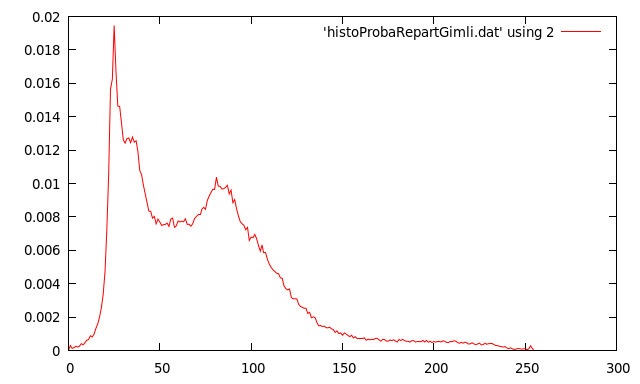
\includegraphics[scale=0.5]{ddpGimliGris.png}\\
\textit{La densité de probabilité de gimli.pgm}
\end{center}
\begin{center}
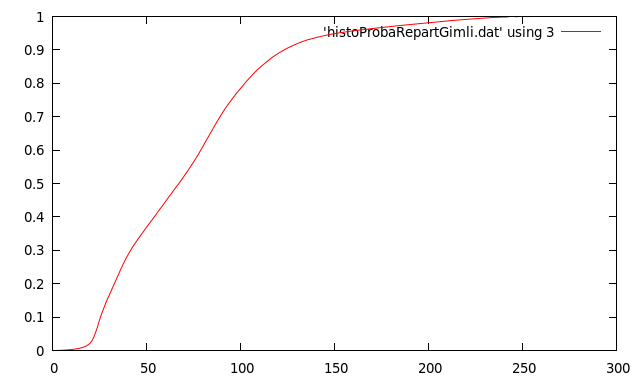
\includegraphics[scale=0.5]{fctionRepartGimliGris.png}\\
\textit{La fonction de répartition de gimli.pgm}
\end{center}
\newpage
\begin{center}
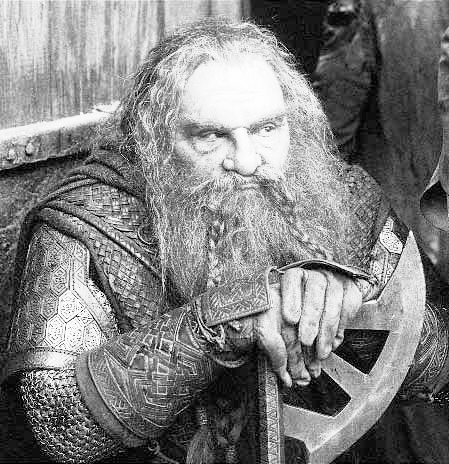
\includegraphics[scale=0.5]{gimliegal.png}
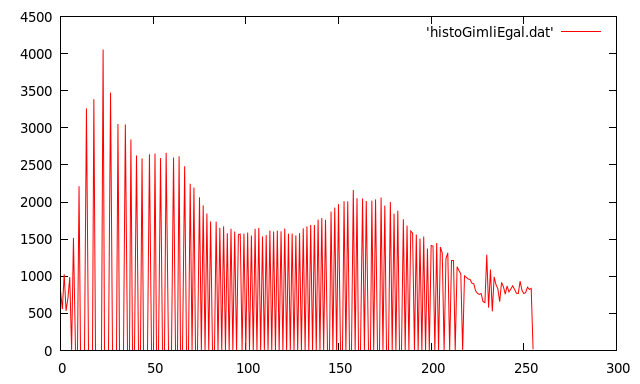
\includegraphics[scale=0.5]{histoGimliEgal.png}\\
\textit{L'image gimli.pgm égalisée, et son histogramme}
\end{center}

\newpage
\section{Spécification d'histogramme}
\paragraph{} L'image référence R lena.pgm a été utilisée, ainsi que gimli.pgm en tant qu'image B.
\begin{center}
\includegraphics[scale=0.25]{gimliA.png}
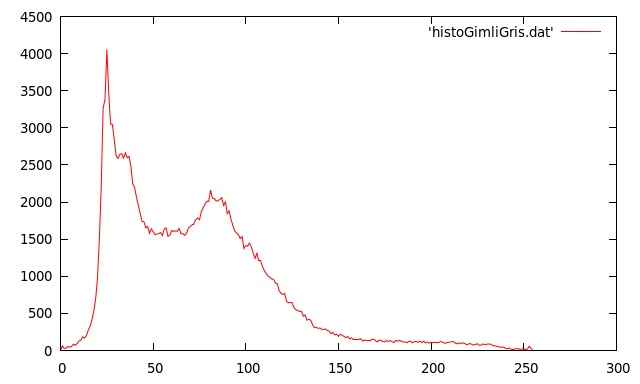
\includegraphics[scale=0.25]{histoGimliGris.png}\\
\textit{L'image gimli.pgm originale, et son histogramme}\\
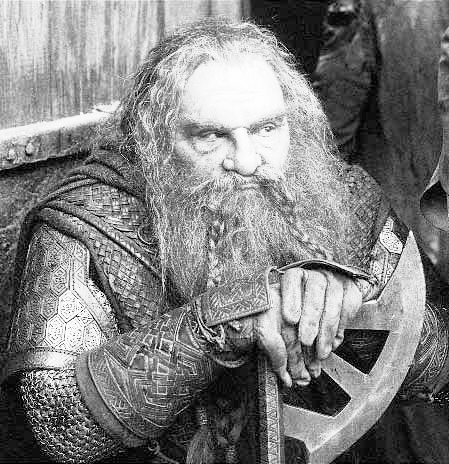
\includegraphics[scale=0.25]{gimliegal.png}
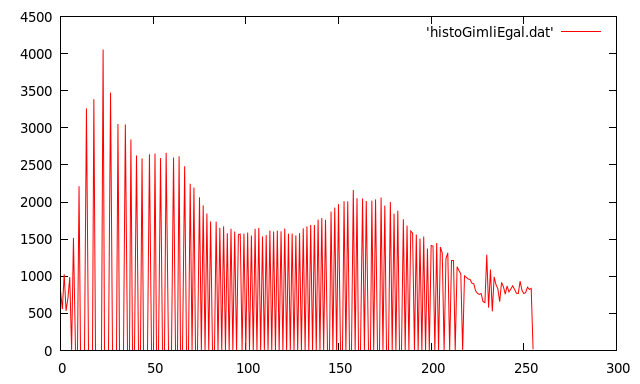
\includegraphics[scale=0.25]{histoGimliEgal.png}\\
\textit{L'image gimli.pgm égalisée, et son histogramme}
\end{center}
\begin{center}
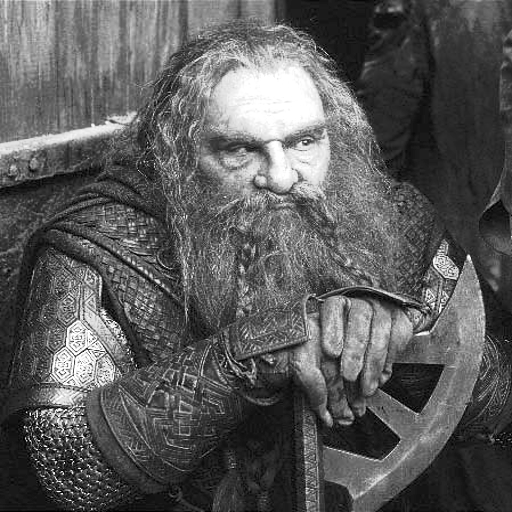
\includegraphics[scale=0.5]{gimlispecifiec.png}
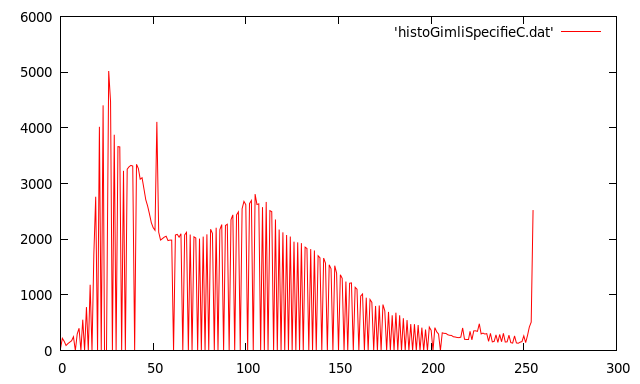
\includegraphics[scale=0.25]{histoGimliSpecifie.png}
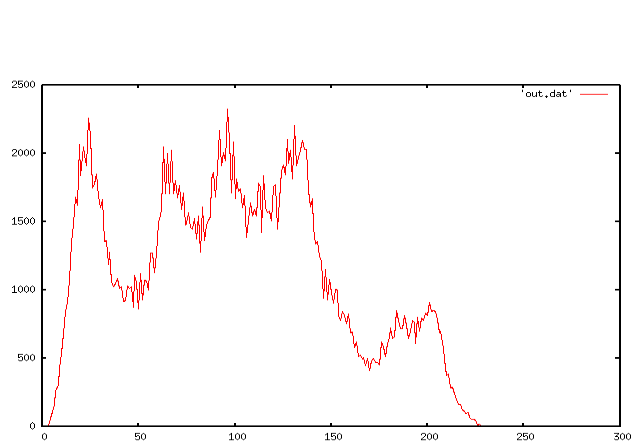
\includegraphics[scale=0.34]{histoLena.png}\\
\textit{L'image gimli.pgm spécifiée, son histogramme et celui de lena.pgm}
\end{center}

\newpage
\section{Bonus}
\begin{center}
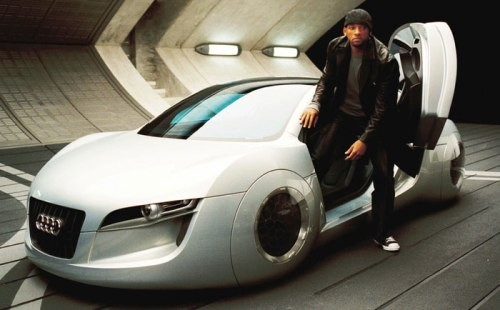
\includegraphics[scale=0.25]{will.png}
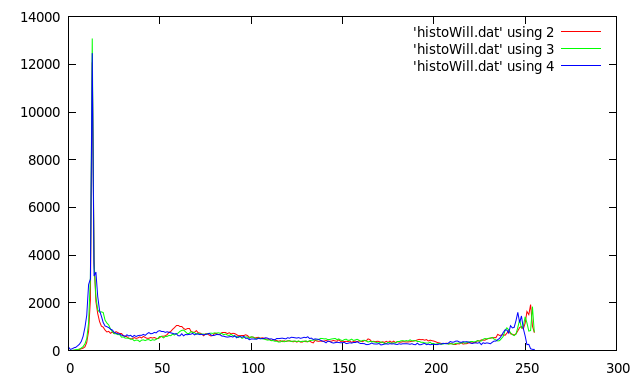
\includegraphics[scale=0.25]{histoWill.png}\\
\textit{L'image willSmith.ppm originale, et son histogramme}
\end{center}
\vspace*{0.5cm}
\begin{center}
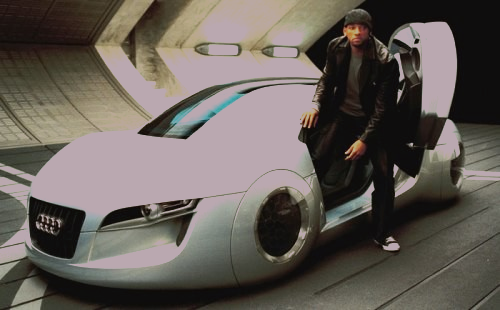
\includegraphics[scale=0.25]{willseuil.png}
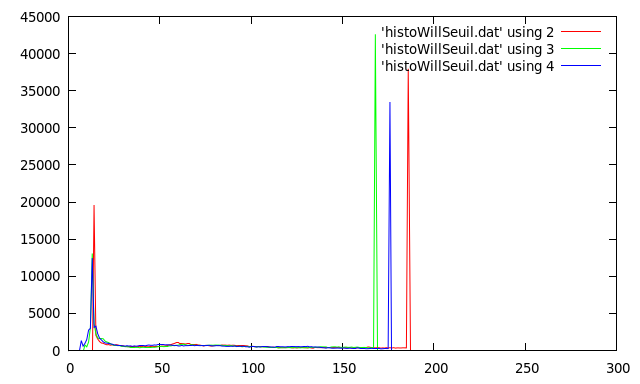
\includegraphics[scale=0.25]{histoWillSeuil.png}\\
\textit{L'image willSmith.ppm seuillée, et son histogramme}
\end{center}
\vspace*{0.5cm}
\begin{center}
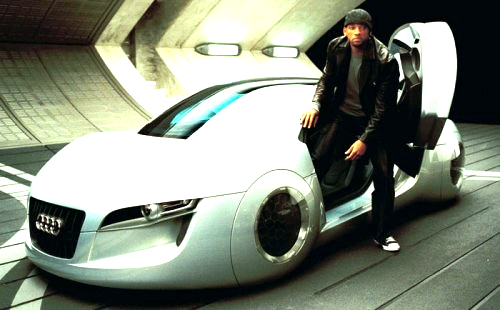
\includegraphics[scale=0.25]{willseuilexpand.png}
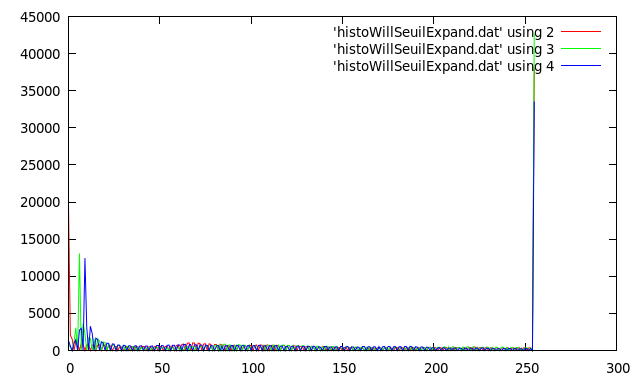
\includegraphics[scale=0.25]{histoWillSeuilExpand.png}\\
\textit{L'image willSmith.ppm après expansion dynamique, et son histogramme}
\end{center}
\vspace*{0.5cm}
\begin{center}
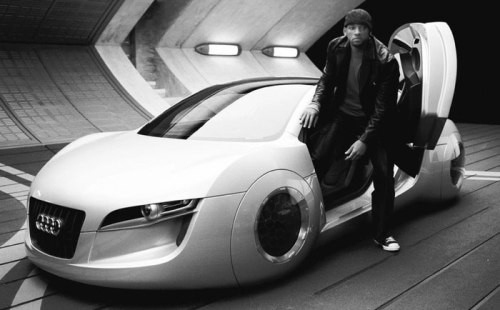
\includegraphics[scale=0.33]{will_pgm.png}
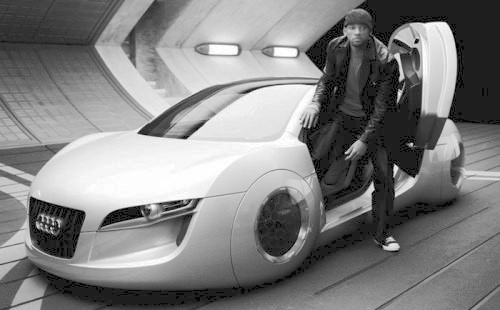
\includegraphics[scale=0.33]{willegal.png}\\
\textit{L'image willSmith.pgm orignale, puis égalisée}
\end{center}

\end{document}